\documentclass{standalone}
\usepackage{tikz}
\usetikzlibrary{patterns,hobby}
\usepackage{pgfplots}
\pgfplotsset{compat=1.6}
\pgfplotsset{ticks=none}

\usetikzlibrary{backgrounds}
\usetikzlibrary{decorations.markings}
\usetikzlibrary{arrows.meta}
\tikzset{>=stealth}

\tikzset{
  clockwise arrows/.style={
    postaction={
      decorate,
      decoration={
        markings,
        mark=between positions 0.1 and 0.9 step 40pt with {\arrow{>}},
   }}}}

\begin{document}

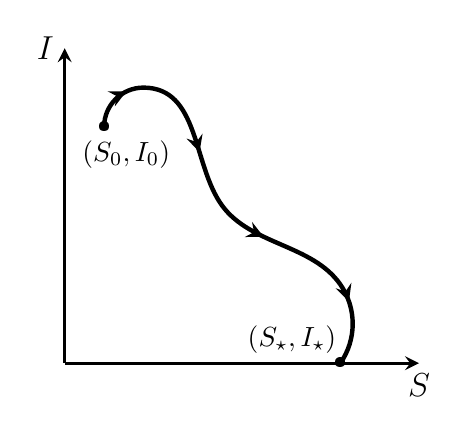
\begin{tikzpicture}
    \draw[->,very thick] (0,0)--(4.5,0) node[below]{\large $S$};
    \draw[->,very thick] (0,0)--(0,4) node[left]{\large $I$};
    %
    \draw (0.5,3) node {\textbullet};
    \draw (3.5,0) node {\textbullet};
    %
    \node  at (0.1,2.95) [anchor=north west] {$(S_0,I_0)$};
    \node  at (2.2,0) [anchor=south west] {$(S_\star,I_\star)$};
    %Hobby package  
    \draw [ultra thick, clockwise arrows] (0.5,3) to [ curve through ={(1,3.5) . . (2,2) . . (3.5,1)}] (3.5,0);% curve 
\end{tikzpicture}
\end{document}